%%
%% copyright quintard julien
%% 
%% kaneton
%% 
%% kaneton.tex
%% 
%% path          /root/data/research/projects/svn/kaneton/projects/k4
%% 
%% made by mycure
%%         quintard julien   [quinta_j@epita.fr]
%% 
%% started on    Mon Feb 21 16:02:54 2005   mycure
%% last update   Sat Mar 12 01:19:34 2005   mycure
%%

\documentclass[10pt,a4wide]{article}
\usepackage[english]{babel}
\usepackage{a4wide}
\usepackage{graphicx}
\usepackage{graphics}
\usepackage{fancyheadings}
\pagestyle{fancy}

\bibliographystyle{plain}

\lhead{\scriptsize{kaneton project}}
\rhead{kaneton}
\rfoot{\scriptsize{EPITA System Lab}}

\title{kaneton}

\author{Julien Quintard - \small{quinta\_j@epita.fr} \\
        Jean-Pascal Billaud - \small{billau\_j@epita.fr} \\ \\
        \small{last updated by} \\
        Julien Quintard - \small{quinta\_j@epita.fr}}

\date{\today}

\begin{document}
\maketitle

\tableofcontents

\newpage

\section{Introduction}

kaneton est un kernel que les \'el\`eves d'epita en specialisation syst\`eme,
r\'eseau et s\'ecurit\'e devront d\'evelopper.

\paragraph{}

L'objectif est d'arriver a d\'evelopper un noyau de syst\`eme d'exploitation
extr\^emement propre au niveau mod\'elisation pour permettre le portage
vers d'autres architectures sans efforts.

\paragraph{}

Le but du projet est de faire acqu\'erir aux \'el\`eves toutes les notions
processeur, syst\`eme, et algorithmique n\'ecessaire pour l'\'elaboration
d'un syst\`eme d'exploitation moderne.

\newpage

\section{Projet}

Il faut savoir que la partie du d\'eveloppement la plus compliqu\'ee est
certainement celle li\'ee directement au processeur car comprendre
et r\'eparer les erreurs est assez fastidieux.

\paragraph{}

L'objectif de ce projet sera donc d'amener l'\'etudiant \`a comprendre le
fonctionnement d'un processeur donn\'e, dans notre cas Intel, puis toutes
les phases de mises en place d'un syst\`eme d'exploitation pour finir
par les drivers et autres installations pour permettre les futures ex\'ecutions
de programmes utilisateurs.

\paragraph{}

L'\'etudiant, \`a la fin de l'ann\'ee, aura d\'evelopp\'e un syst\`eme
d'exploitation de type micro-kernel complet et portable comprenant une
gestion de m\'emoire, une gestion des processus avec threads, une gestion
des entr\'ees/sorties, une gestion des communication inter-processus
mais aussi une gestion des p\'eriph\'eriques avec plusieurs drivers:
r\'eseau, disque dur, file systems etc..

\paragraph{}

L'\'etudiant aura donc la possibilit\'e d'\'etudier le fonctionnement d'un
processeur, de pratiquer plusieurs langages de bas niveau notamment
l'assembleur intel et le C. Une fois ces \'etapes que l'on pourrait
qualifier de ``hardware'' d\'epass\'ees, l'\'etudiant devra faire face
\`a des probl\'ematiques de plus haut niveau comme par exemple la gestion
m\'emoire, le scheduling, la portabilit\'e, et bien d'autres designs pour la
gestion d'\'el\'ements noyaux.

\newpage

\section{Organisation}

Le projet kaneton est decoup\'e en sous projets de sorte que l'etudiant
valide bien chaque notion: mode d'adressages, gestion memoire, gestion
des processus etc..

\paragraph{}

Voyons donc d\'esormais la liste des sous projets, des \'etapes que
l'\'etudiant devra suivre.

\newpage

\subsection{KAN1: Mise en place du kernel}

\subsubsection{k0}

D\'eveloppement d'un bootstrap. L'\'etudiant sera amen\'e \`a comprendre
un mode d'adressage du processeur et d'en installer un nouveau.

\vspace{5cm}

\begin{figure}[h]
\centerline{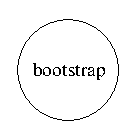
\includegraphics{figures/k0.eps}}
\end{figure}

\newpage

\subsubsection{k1}

D\'eveloppement d'un bootloader. Celui ci devra mettre en place un nouveau
mode d'adressage et installer une configuration m\'emoire satisfaisante pour
la future ex\'ecution du kernel.

\vspace{5cm}

\begin{figure}[h]
\centerline{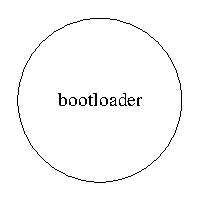
\includegraphics{figures/k1.eps}}
\end{figure}

\newpage

\subsubsection{k2}

Lancement du kernel et mise en place d'un certain nombre de gestionnaires:
m\'emoire physique, interruptions etc.. et certains drivers basiques:
timer, console, clavier etc..

\vspace{5cm}

\begin{figure}[h]
\centerline{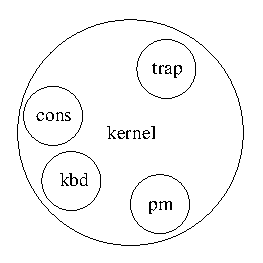
\includegraphics{figures/k2.eps}}
\end{figure}

\newpage

\subsection{KAN2: Gestion des ressources et IPC}

\subsubsection{k3}

Mise en place du gestionnaire de m\'emoire virtuelle.

\vspace{5cm}

\begin{figure}[h]
\centerline{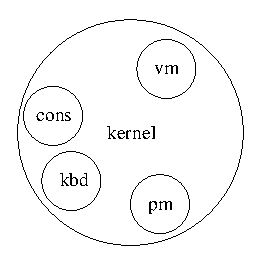
\includegraphics{figures/k3.eps}}
\end{figure}

\newpage

\subsubsection{k4}

Mise en place de la gestion des processus avec gestion des threads.

\vspace{5cm}

\begin{figure}[h]
\centerline{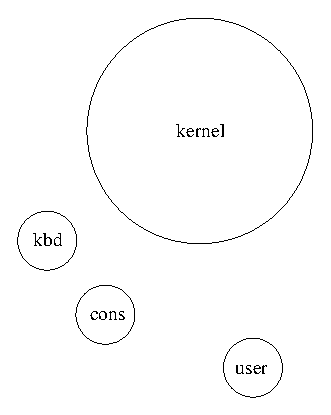
\includegraphics{figures/k4.eps}}
\end{figure}

\newpage

\subsubsection{k5}

D\'eveloppement des IPC et d\'eveloppement d'un systeme de buffering de
messages.

\vspace{5cm}

\begin{figure}[h]
\centerline{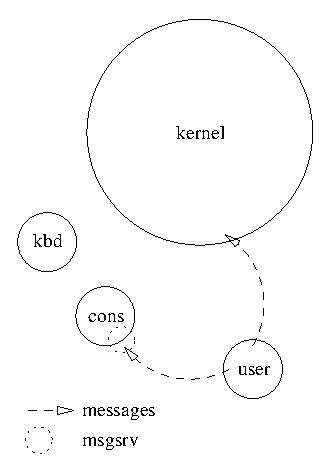
\includegraphics{figures/k5.eps}}
\end{figure}

\newpage

\subsection{KAN3: Syst\`eme de fichiers}

\subsubsection{k6}

D\'eveloppement d'un driver IDE et d'une gestion des partitions.

\vspace{5cm}

\begin{figure}[h]
\centerline{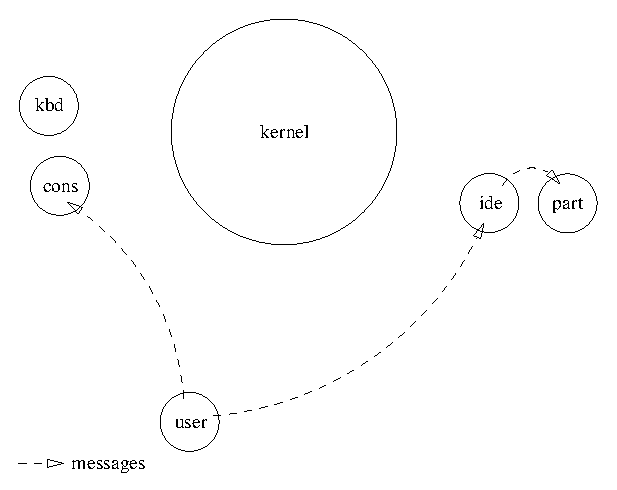
\includegraphics{figures/k6.eps}}
\end{figure}

\newpage

\subsubsection{k7}

D\'eveloppement d'un gestionnaire de p\'eriph\'eriques. D\'eveloppement
d'une libc avec les librairies utilisateurs: crt etc..

\vspace{5cm}

\begin{figure}[h]
\centerline{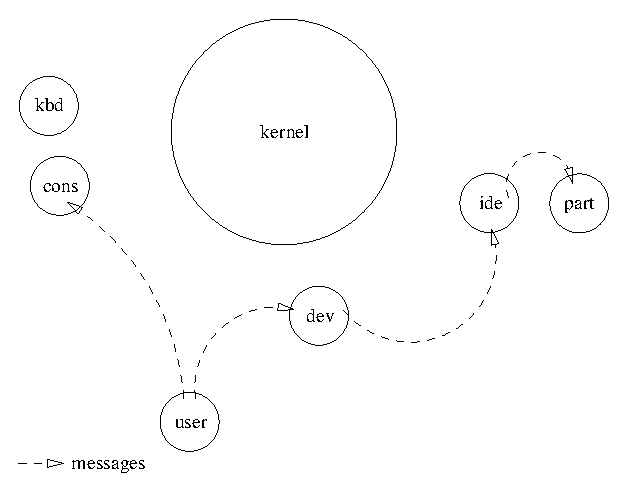
\includegraphics{figures/k7.eps}}
\end{figure}

\newpage

\subsubsection{k8}

D\'eveloppement d'un syst\`eme de fichier et du syst\`eme de fichier
g\'en\'erique VFS.

\vspace{5cm}

\begin{figure}[h]
\centerline{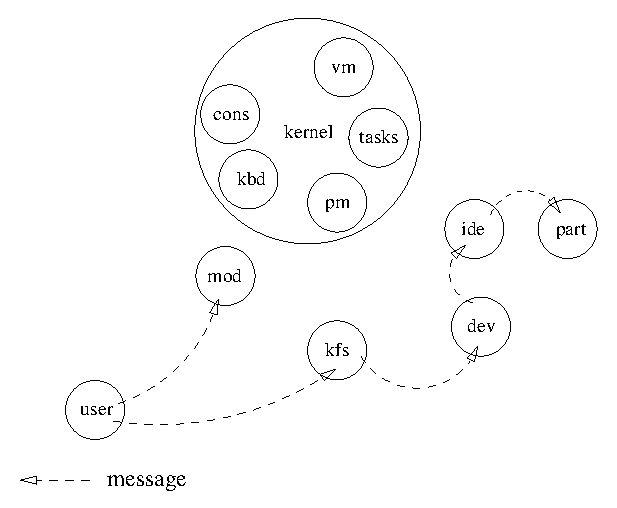
\includegraphics{figures/k8.eps}}
\end{figure}

\newpage

\subsection{KAN4: R\'eseau}

\subsubsection{k9}

D\'eveloppement du driver pci et du driver r\'eseau.

\vspace{5cm}

\begin{figure}[h]
\centerline{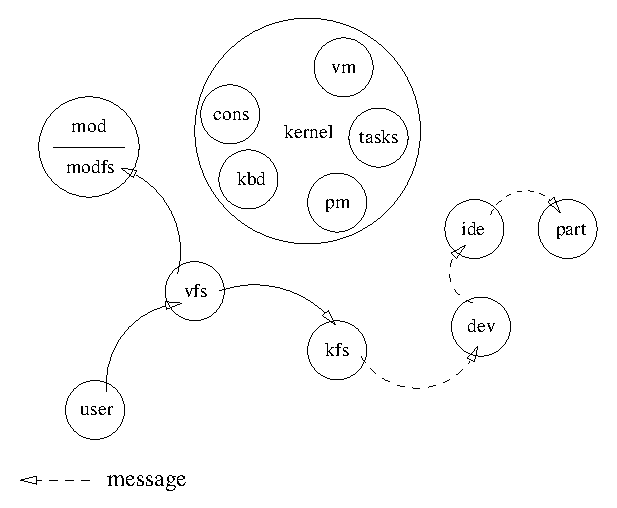
\includegraphics{figures/k9.eps}}
\end{figure}

\newpage

\subsubsection{k10}

D\'eveloppement d'une stack TCP/IP.

\vspace{5cm}

\begin{figure}[h]
\centerline{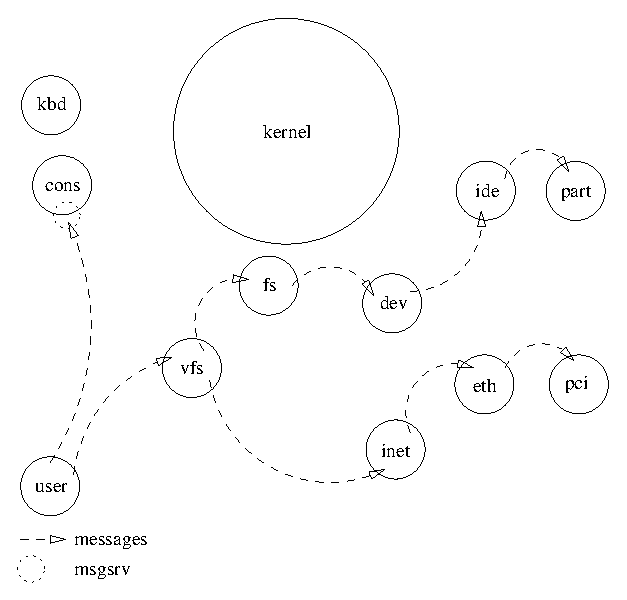
\includegraphics{figures/k10.eps}}
\end{figure}

\newpage

\section{D\'eroulement d'un projet}

Chaque projet se d\'eroule de la facon suivante:

\begin{enumerate}

\item \textbf{Pr\'esentation du projet}: explication des objectifs \`a
      atteindre, des notions \`a acqu\'erir, de la mod\'elisation propos\'ee
      etc..

\item \textbf{Tp}: durant le projet, des tps seront organis\'es,
      g\'en\'eralement une sc\'eance toute les semaines, afin que vous
      puissiez poser vos questions.

\item \textbf{Soutenance}: \`a l'issue de chaque p\'eriode de projet, une
      soutenance aura lieu afin d'\'evaluer le travail du groupe. Attention,
      la notation sera bas\'ee sur les r\'eponses de chaque membre du groupe.
      En d'autres termes, si plusieurs personnes dans le groupe ne savent
      pas r\'epondre la note s'en verra recalcul\'ee.

\item \textbf{Partiel}: un partiel aura lieu pour valider vos connaissances
      sur la totalit\'e des notions vues jusque l\`a.

\end{enumerate}

\paragraph{}

Il est important de savoir qu'aucun support de cours ne sera fourni. La
pr\'esentation du projet inclus un cours sur les notions \`a comprendre
et \`a connaitre. Les \'etudiants sont donc fortement invit\'es \`a
assister aux cours et \`a prendre des notes pour ne pas perdre de temps
durant le d\'eveloppement du projet.

\paragraph{}

Le sujet sera le seul document fourni et contiendra en plus de la description
du projet, la liste des documentations \`a lire pour r\'eussir le projet.
Bien entendu, l'\'etudiant qui aura assimil\'e les notions abord\'ees en
cours n'aura quasiment aucun document \`a lire.

\paragraph{}

Certains projets sont destin\'es \`a initier les \'etudiants \`a la
mod\'elisation dans un kernel. Dans ces projets particuliers, nous
vous invitons \`a suivre notre mod\'elisation. N\'eanmoins vous
pourrez tout \`a fait prendre la d\'ecision d'impl\'ementer votre
propre mod\'elisation. Dans ce cas, vous devrez nous fournir une documentation
claire et pr\'ecise expliquant vos choix. Si votre mod\'elisation est
intelligente et apporte des inovations par rapport \`a celle fournie,
nous prendrons certainement la d\'ecision d'utiliser votre impl\'ementation.
Libre \`a vous donc de nous \'epater.

\end{document}
